% 实验二：使用 Wireshark 分析 Web 访问过程流量
% 在此填写 DNS、ARP、TCP、HTTP、Follow TCP Stream 和 Cookie 分析。
\section{实验二：使用 Wireshark 分析 Web 访问过程流量}

\subsection{实验目的}
\begin{enumerate}
    \item 学习并掌握Wireshark在网络流量分析中的作用，以及如何通过它来捕获和分析网络数据包;
    \item 通过实际操作，观察并分析域名解析过程中涉及的IP包，理解DNS请求和响应的格式和内容,以及它是如何将域名转换为IP地址的;
    \item 观察并解释Client与www.imool.com.cn之间TCP连接的建立和拆除过程，包括三次握手和四次挥手;
    \item 使用Wireshark的协议流追踪功能，提取并分析Web访问过程中产生的Cookie信息
\end{enumerate}

\subsection{实验配置}
本次实验采用 Oracle VirtualBox 搭建实验环境，OpenWRT路由器通过三个接口分别和Client、Web Server、DNS相连，具体网络拓扑的配置如下：
\begin{table}[H]
    \centering
    \caption{实验二各虚拟机网络接口及 IP 地址配置}
    \label{tab:exp2_network}
    \begin{tabular}{cccc}
        \toprule
        虚拟机 & Linux 内网卡名 & IP 地址 & 默认网关 \\
        \midrule
        Client      & \texttt{enp0s3} & \texttt{192.168.3.10/24}  & \texttt{192.168.3.1} \\
        DNS Server  & \texttt{enp0s3} & \texttt{192.168.2.53/24}  & \texttt{192.168.2.1} \\
        Web Server  & \texttt{enp0s3} & \texttt{192.168.4.105/24} & \texttt{192.168.4.1} \\
        OpenWRT     & \texttt{eth1}   & \texttt{192.168.4.1/24}   & -- \\
        OpenWRT     & \texttt{eth2}   & \texttt{192.168.3.1/24}   & -- \\
        OpenWRT     & \texttt{eth3}   & \texttt{192.168.2.1/24}   & -- \\
        OpenWRT     & \texttt{eth0}   & DHCP                      & -- \\
        \bottomrule
    \end{tabular}
\end{table}
网络拓扑如图所示：
\begin{figure}[H]
    \centering
    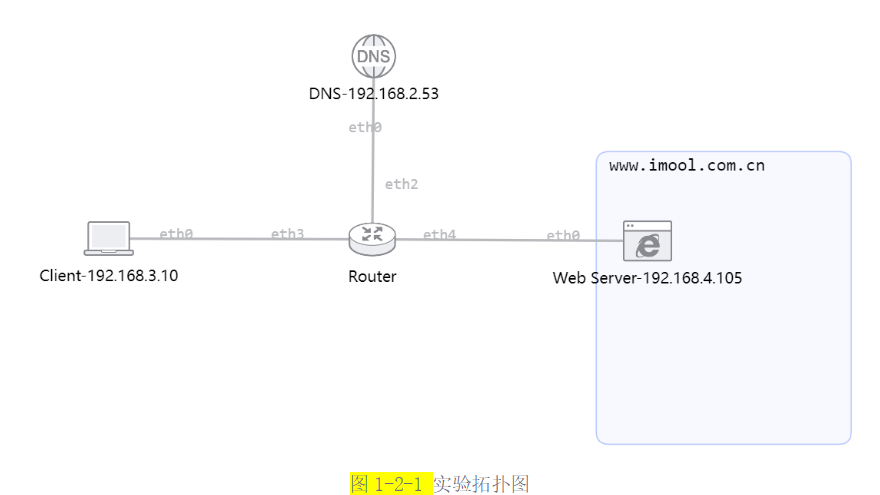
\includegraphics[width=0.8\textwidth]{figures/exp2_network.png}
    \caption{实验二网络拓扑图}
    \label{fig:exp2_network}
\end{figure}
\subsection{实验过程}
\subsubsection{配置 Web Server}
在 Web Server 主机 192.168.4.105 上启动 HTTP 服务。
由于系统中未安装 Apache 或 Nginx，因此使用 Python 自带的 HTTP Server 建立简单的 Web 服务。
执行：
\begin{lstlisting}[language=bash,caption={建立简单的 Web 服务}]
sudo python3 -m http.server 80 --bind 0.0.0.0
ss -lntp
\end{lstlisting}
查看端口监听状态，可以看到 0.0.0.0:80 已处于监听状态，
说明 Web Server 已成功提供 HTTP 服务。
\begin{figure}[H]
    \centering
    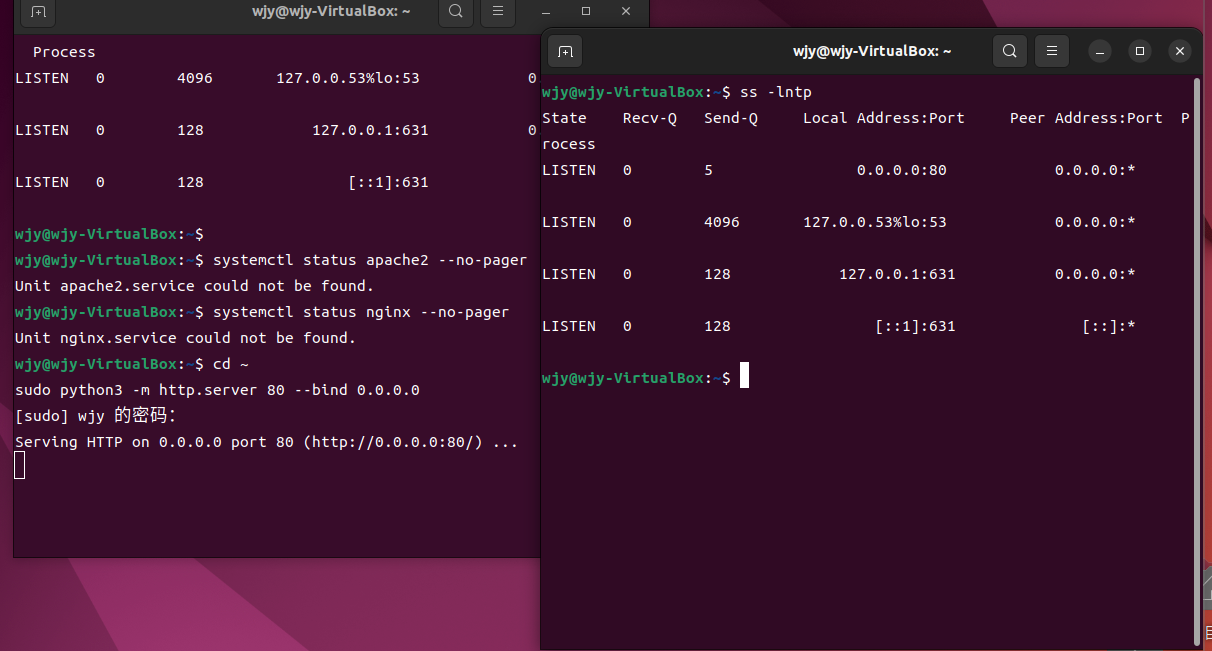
\includegraphics[width=0.8\textwidth]{figures/exp2_http.png}
    \caption{Web Server 启动 HTTP 服务截图}
    \label{fig:exp2_http}
\end{figure}

\subsubsection{配置 DNS Server}
在虚拟机DNS Server上打开终端，使用nano编辑器创建配置文件：
\begin{lstlisting}[language=bash,caption={创建DNS配置文件}]
cat > ~/imool-dnsmasq.conf <<'EOF'
listen-address=192.168.2.53
bind-interfaces
address=/www.imool.com.cn/192.168.4.105
no-resolv
EOF  
\end{lstlisting}
检查配置文件的语法，如下：
\begin{lstlisting}[language=bash,caption={检查DNS配置文件语法}] 
sudo dnsmasq --test --conf-file="$HOME/imool-dnsmasq.conf"
\end{lstlisting}
在确认后，启用DNS服务，如下：
\begin{lstlisting}[language=bash,caption={启用DNS服务}]
sudo dnsmasq --no-daemon --conf-file="$HOME/imool-dnsmasq.conf"
\end{lstlisting}

此时 DNS Server 可以响应 Client 对 www.imool.com.cn 的解析请求，
并返回 Web Server 的 IP 地址 192.168.4.105。
\begin{figure}[H]
    \centering
    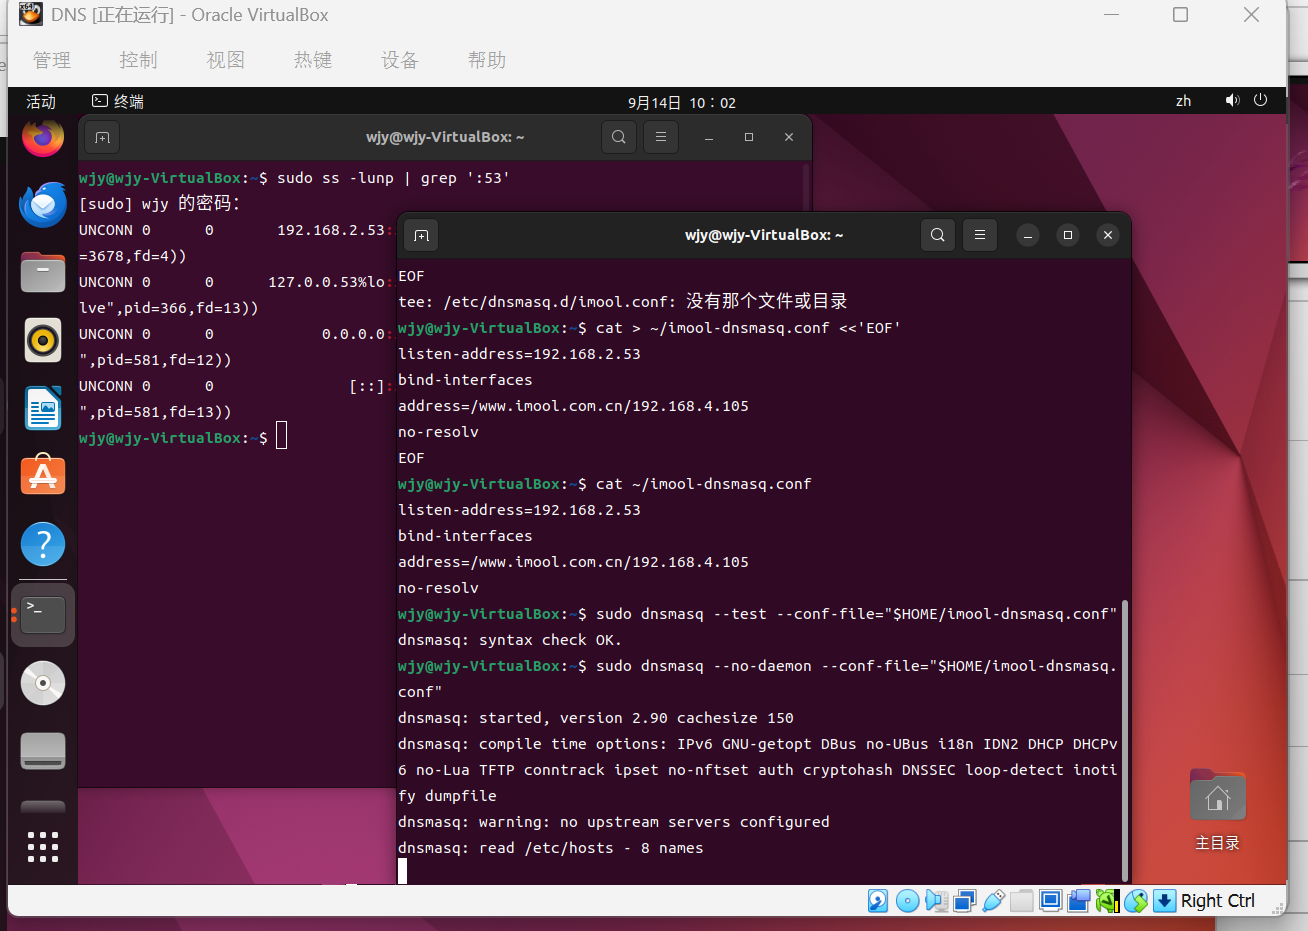
\includegraphics[width=0.8\textwidth]{figures/exp2_dns.png}
    \caption{DNS Server 启动截图}
    \label{fig:exp2_dns}
\end{figure}

\subsubsection{配置 Client 并启动 Wireshark}
在 Client 上启动 Wireshark，并选择 enp0s3 接口监听网络流量。
为尽可能完整地观察 ARP 和 DNS 解析过程，在访问网站前清除相关缓存：
\begin{lstlisting}[language=bash,caption={清除 DNS 缓存}]
sudo ip neigh flush all
sudo resolvectl flush-caches
\end{lstlisting}
之后开始 Wireshark 抓包:
\begin{lstlisting}[language=bash,caption={启动 Wireshark 抓包}]sudo wireshark &
sudo wireshark
\end{lstlisting}

在Client上先运行Wireshark，选择监听以太网网卡eth0的所有流量；
在Client上通过浏览器访问$$ http://www.imool.com.cn $$，然后结束访问该网站；
\begin{figure}[H]
    \centering
    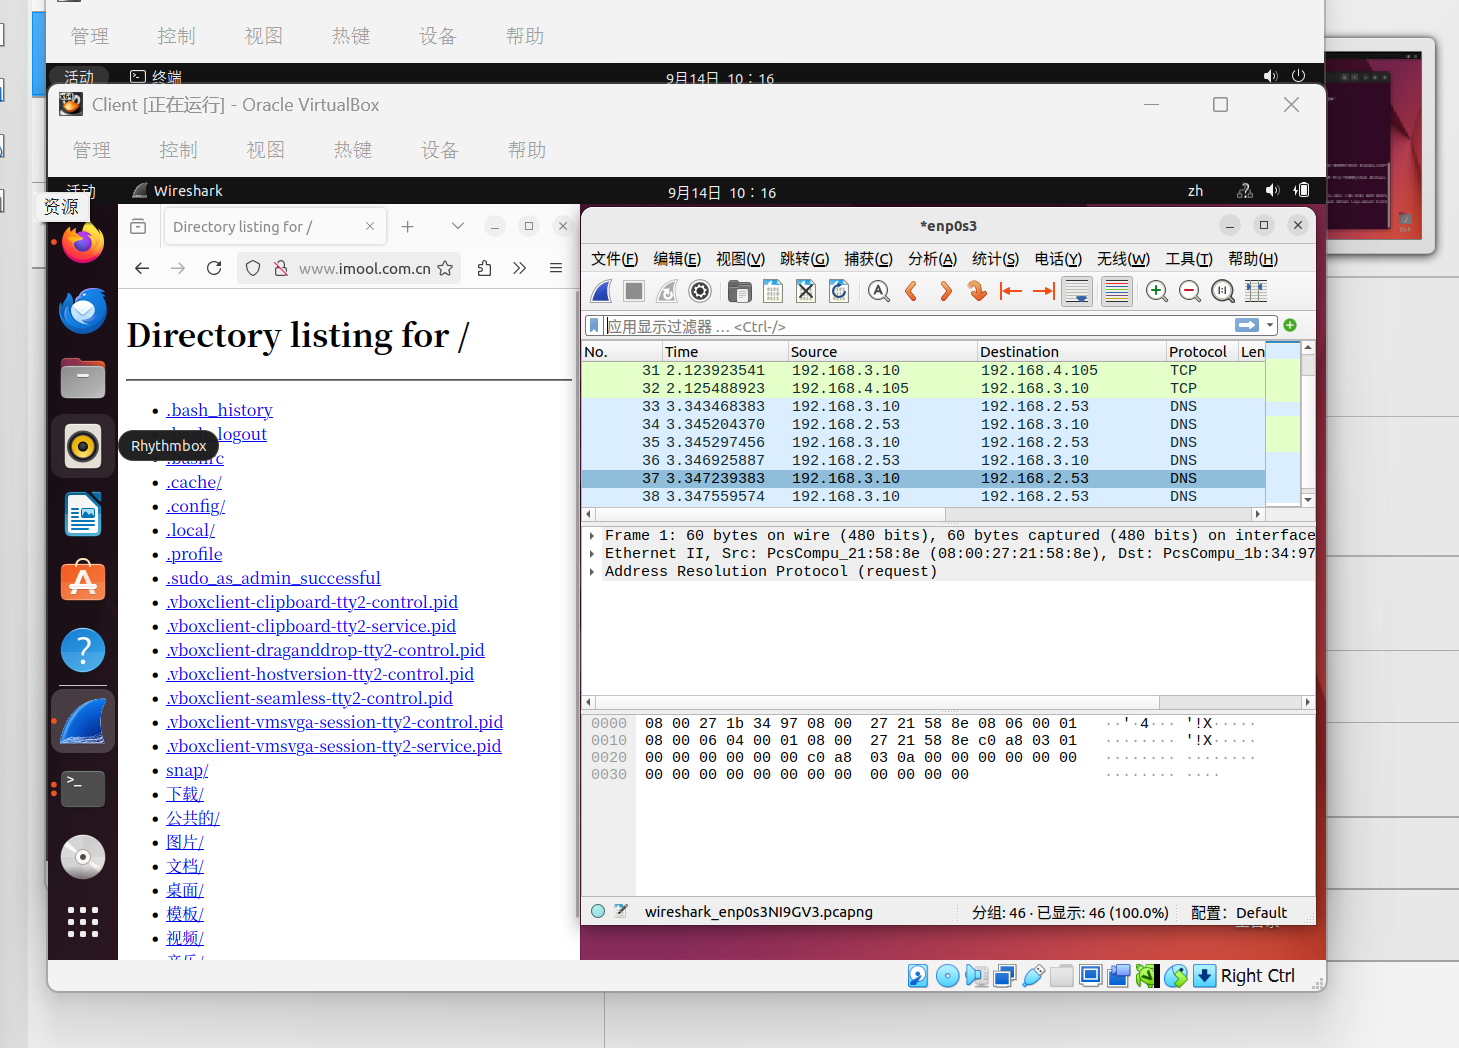
\includegraphics[width=0.8\textwidth]{figures/exp2_wireshark.png}
    \caption{Wireshark抓包截图}
    \label{fig:exp2_wireshark}
\end{figure}


\subsubsection{抓取相关的协议流量}
抓取相关的DNS流量，如下：
\begin{figure}[H]
    \centering
    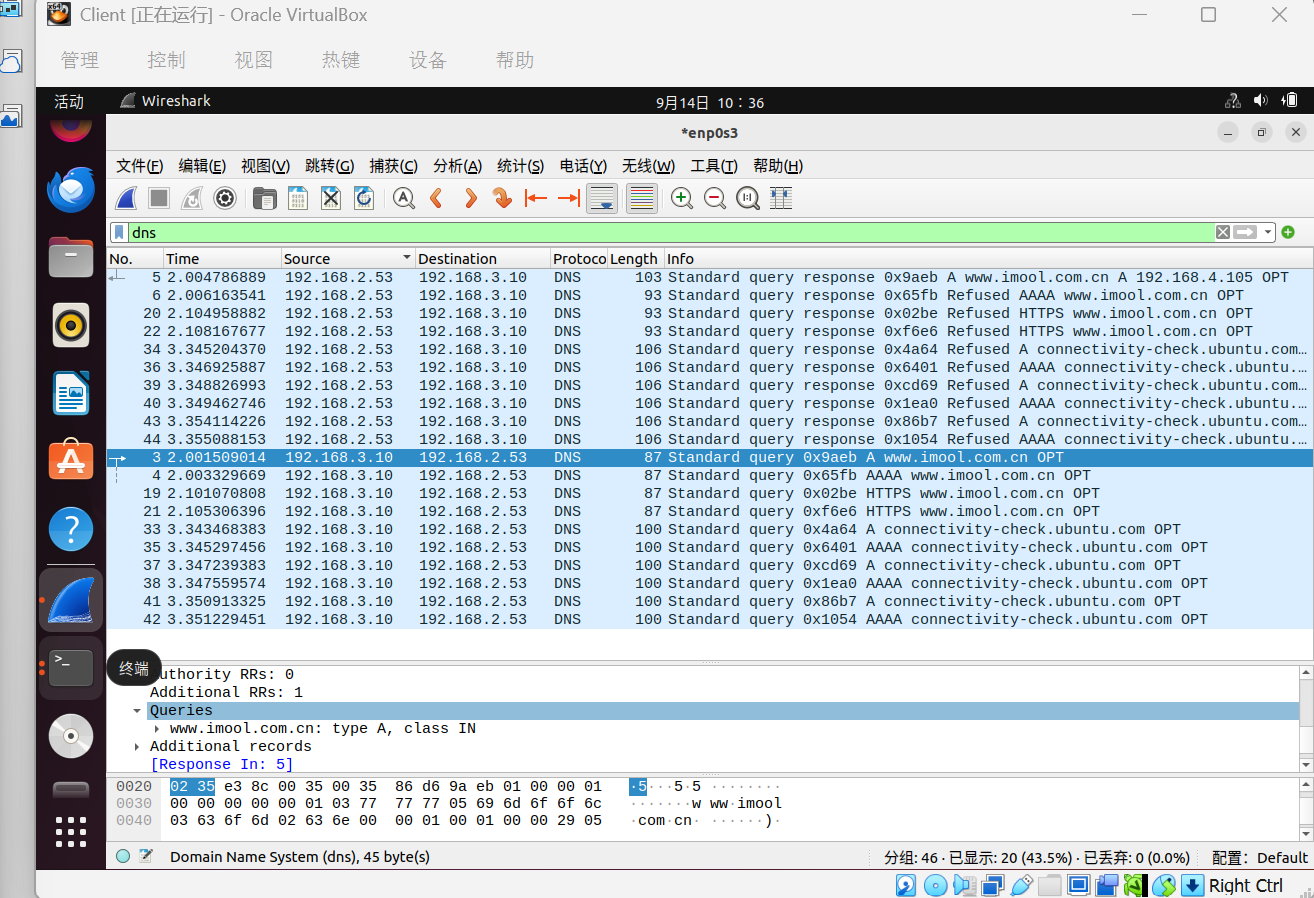
\includegraphics[width=0.8\textwidth]{figures/exp2_dns_1.png}
    \caption{DNS流量截图1}
    \label{fig:exp2_dns_1}
\end{figure}

\begin{figure}[H]
    \centering
    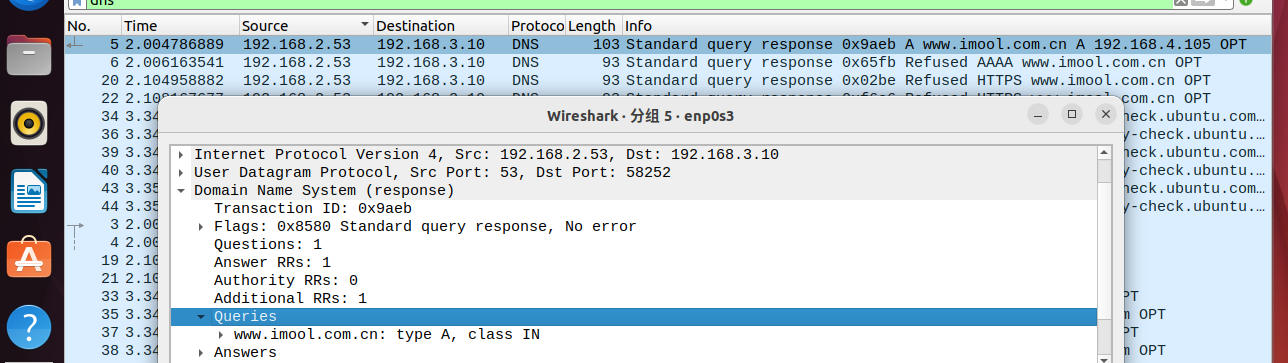
\includegraphics[width=0.8\textwidth]{figures/exp2_dns_2.png}
    \caption{DNS流量截图2}
    \label{fig:exp2_dns_2}
\end{figure}

抓取相关的ARP流量，如下：
\begin{figure}[H]
    \centering
    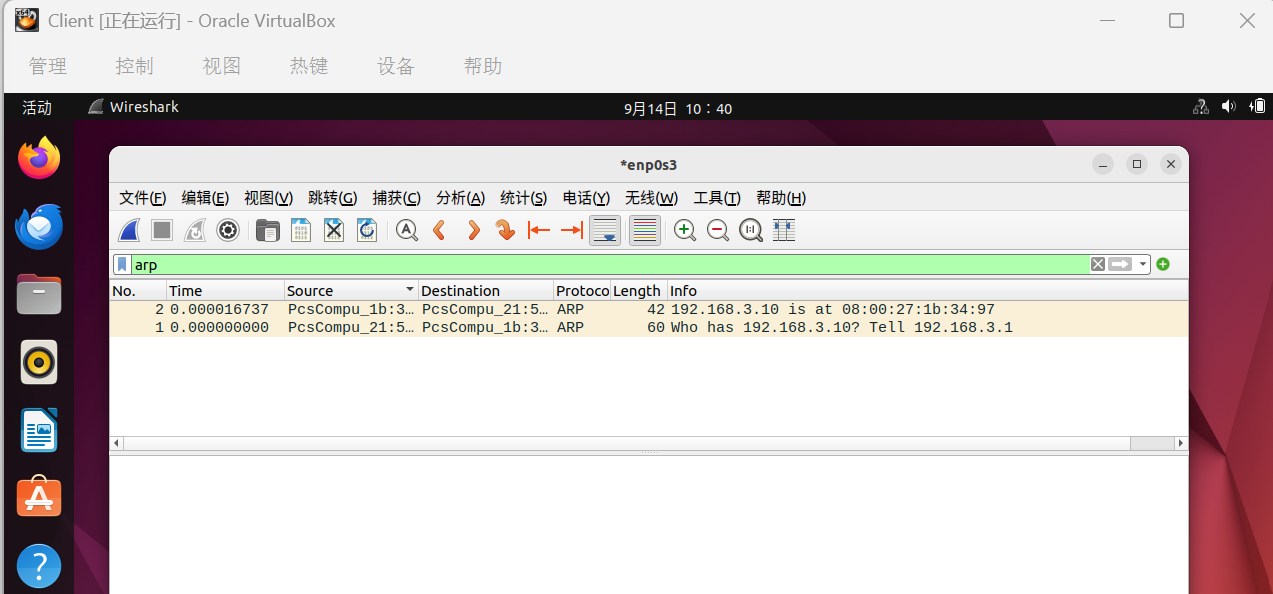
\includegraphics[width=0.8\textwidth]{figures/exp2_arp.png}
    \caption{ARP流量截图}
    \label{fig:exp2_arp}
\end{figure}

抓取相关的TCP流量，如下：
\begin{figure}[H]
    \centering
    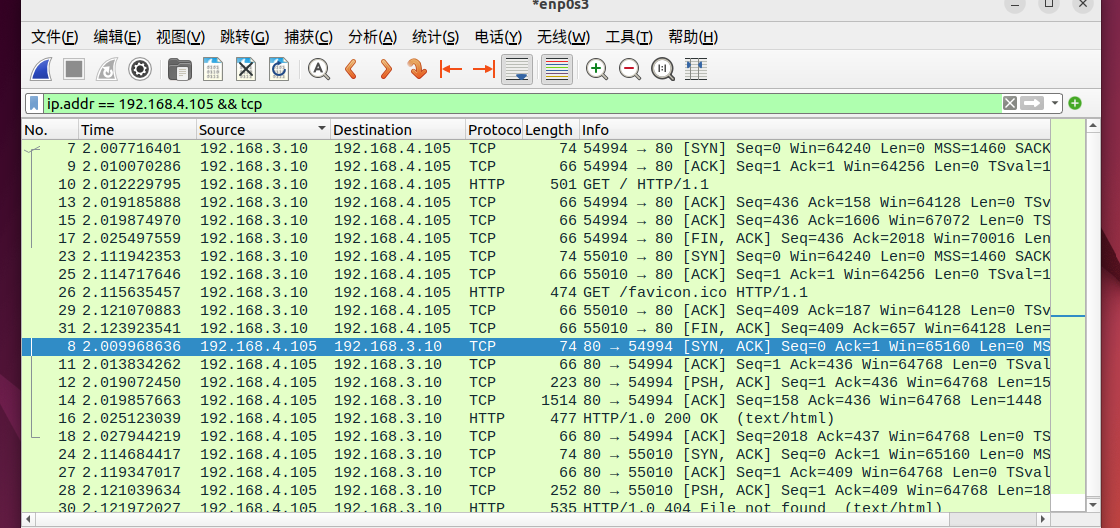
\includegraphics[width=0.8\textwidth]{figures/exp2_tcp.png}
    \caption{TCP流量截图}
    \label{fig:exp2_tcp}
\end{figure}

抓取相关的HTTP流量，如下：
\begin{figure}[H]
    \centering
    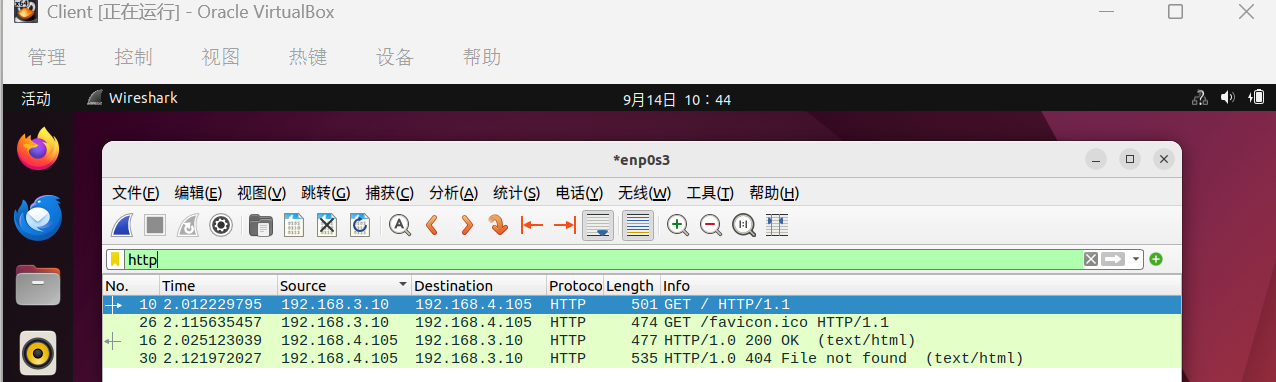
\includegraphics[width=0.8\textwidth]{figures/exp2_http_1.png}
    \caption{HTTP流量截图1}
    \label{fig:exp2_http_1}
\end{figure}

\begin{figure}[H]
    \centering
    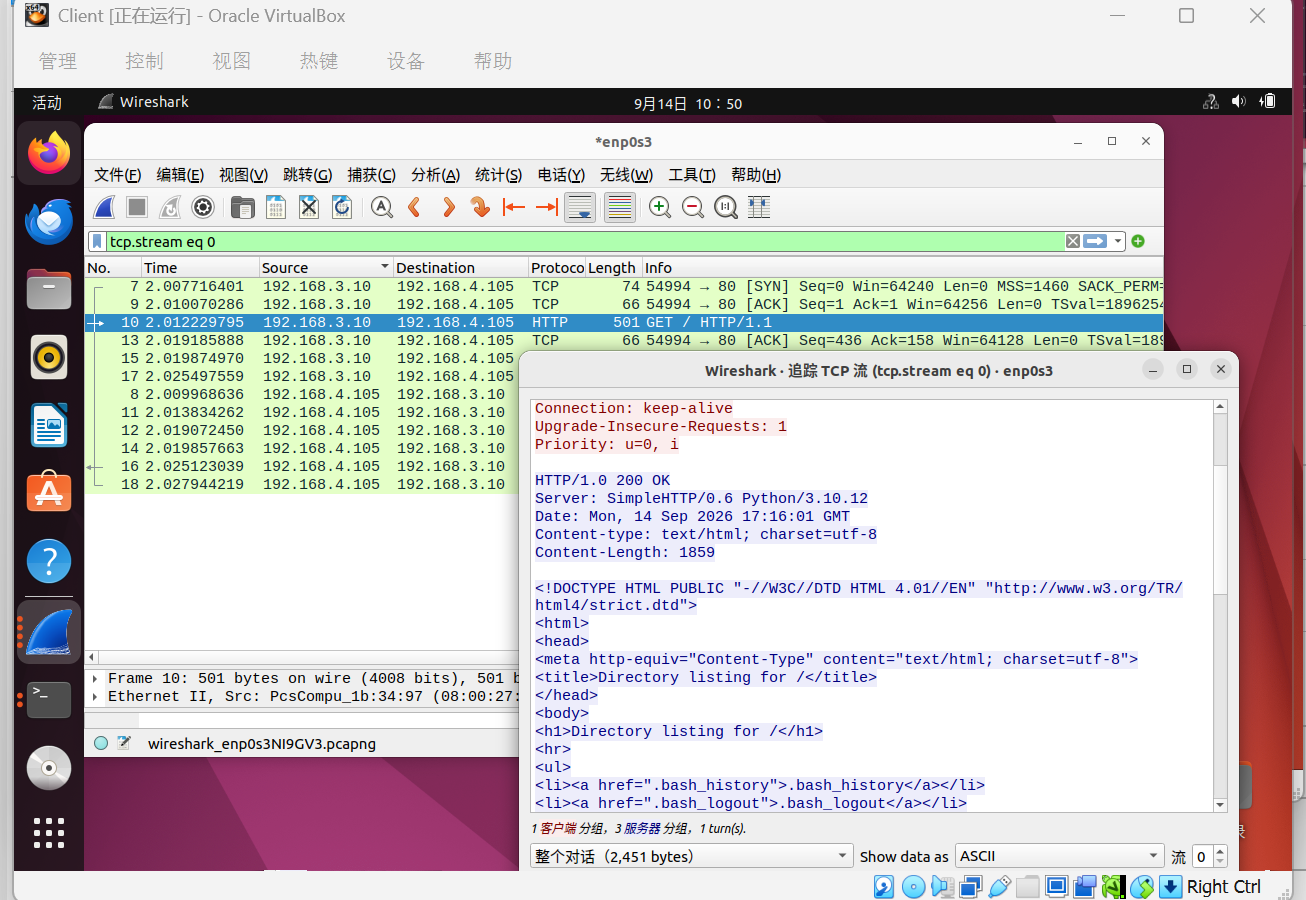
\includegraphics[width=0.8\textwidth]{figures/exp2_http_2.png}
    \caption{HTTP流量截图2}
    \label{fig:exp2_http_2}
\end{figure}

发现上述图片中没有cookie，于是自己手写添加一个，
创建一个简单的服务器：
\begin{lstlisting}[language=python,caption={创建简单的服务器}]
nano ~/cookie_server.py
\end{lstlisting}
写入：
\begin{lstlisting}[language=python,caption={写入简单的服务器}]
from http.server import HTTPServer, SimpleHTTPRequestHandler

class CookieHandler(SimpleHTTPRequestHandler):
    def end_headers(self):
        self.send_header("Set-Cookie", "username=wjy; Path=/")
        super().end_headers()

server = HTTPServer(("0.0.0.0", 80), CookieHandler)

print("HTTP server running on port 80...")
server.serve_forever()
\end{lstlisting}
保存以后运行：
\begin{lstlisting}[language=bash,caption={运行简单的服务器}]
sudo python3 ~/cookie_server.py
\end{lstlisting}

最后重新执行：
wireshark抓包，firebox访问 $$ http://www.imool.com.cn $$ ，
刷新页面，停止抓包，最后是找HTTP，再使用追踪TCP流查看cookie,如下图所示：
\begin{figure}[H]
    \centering
    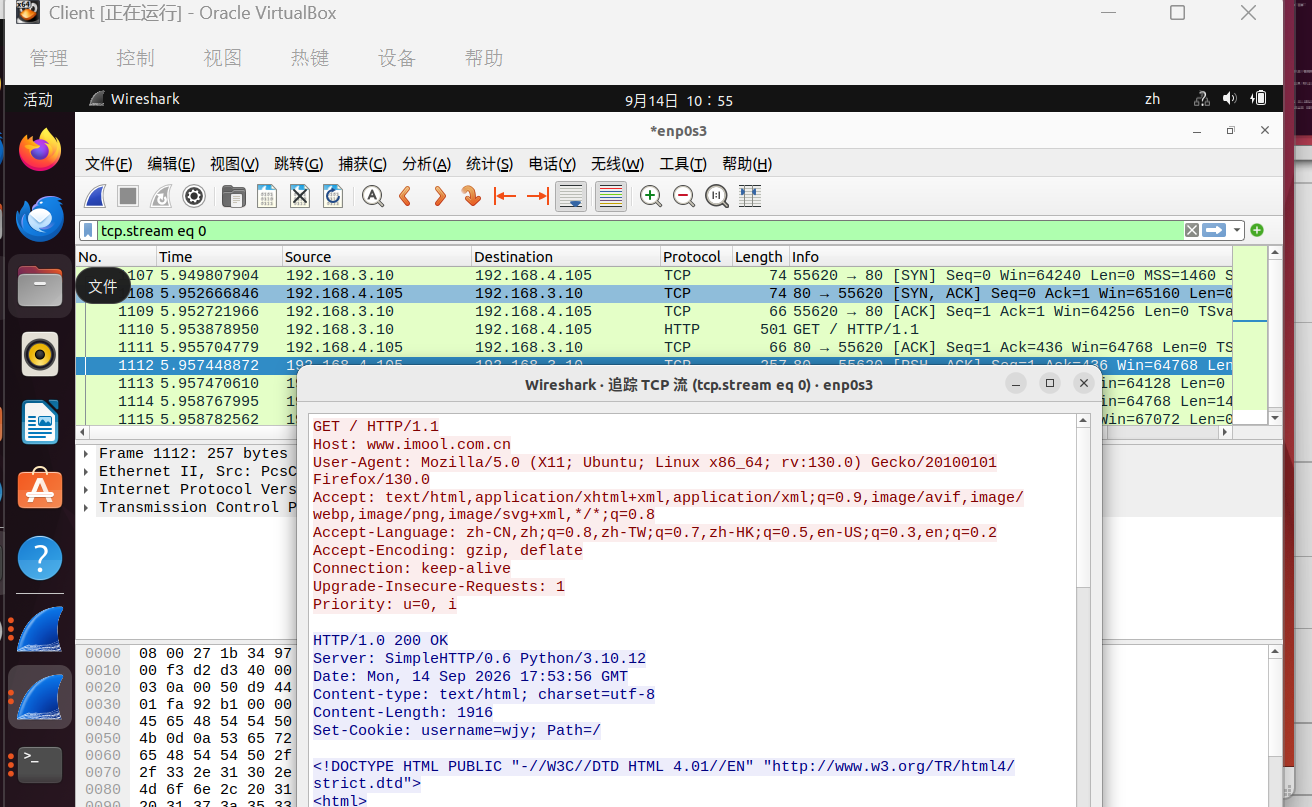
\includegraphics[width=0.8\textwidth]{figures/exp2_cookie.png}
    \caption{HTTP流量截图3}
    \label{fig:exp2_cookie}
\end{figure}

\subsection{特别关注的相关问题}
\subsubsection{域名解析过程涉及哪些IP包，请求和响应分别是什么}
虚拟机 Client （192.168.3.10） 向 DNS Server （192.168.2.53） 发送 DNS 查询请求，
请求解析 www.imool.com.cn；DNS Server 返回请求的响应，将该域名解析为 Web Server 地址 192.168.4.105

\subsubsection{ARP解析过程中，网关的MAC地址是什么}
根据 Wireshark 捕获到的 ARP Response（ARP 响应），默认网关 192.168.3.1 的 MAC 地址为：\\
08:00:27:1b:34:97

\subsubsection{Client 与 www.imool.com.cn 的连接建立和拆除过程}
TCP 连接建立采用三次握手：
192.168.3.10 → 192.168.4.105    [SYN]
192.168.4.105 → 192.168.3.10    [SYN, ACK]
192.168.3.10 → 192.168.4.105    [ACK]

TCP 连接拆除采用四次挥手为：
Client → Web Server       FIN, ACK
Web Server → Client       ACK
Web Server → Client       FIN, ACK
Client → Web Server       ACK

\subsubsection{使用 Wireshark 的协议流追踪功能提取 Cookie 信息}
在 Wireshark 中选择 HTTP 数据流并使用 TCP Stream（TCP 流）追踪功能，
可以观察到服务器返回的：
\begin{lstlisting}[language=bash,caption={cookie的显示}]
Set-Cookie: username=wjy; Path=/
\end{lstlisting}
其中 Cookie 名称为 username，值为 wjy，路径为 /。

\subsection{实验小结}
这一小节实验在实验一网络拓扑的基础上重新配置 DNS Server 和 Web Server，
并利用 OpenWRT 实现不同子网之间的路由通信。
通过 Wireshark 对访问 www.imool.com.cn 的全过程进行抓包，
观察了 DNS 域名解析、ARP 地址解析、TCP 三次握手和四次挥手以及 HTTP 请求和响应过程，
并通过 TCP 流追踪提取了 Cookie 信息。
通过本实验，我们对浏览器访问一个 Web 网站过程中各层协议之间的配合关系有了更加直观的认识。
